\documentclass{thesisclass}
% Based on thesisclass.cls of Timo Rohrberg, 2009
% ----------------------------------------------------------------
% Thesis - Main document
% ----------------------------------------------------------------


%% -------------------------------
%% |  Information for PDF file   |
%% -------------------------------
\hypersetup{
 pdfauthor={Daniel Lipp},
 pdftitle={EAs for Partition},
 pdfsubject={?},
 pdfkeywords={?}
}


%% ---------------------------------
%% | Information about the thesis  |
%% ---------------------------------

\newcommand{\myname}{Daniel Lipp}
\newcommand{\mytitle}{Theoretical and empirical runtime analysis of evolutionary algorithms for the PARTITION problem}
\newcommand{\myinstitute}{Chair of algorithms for intelligent systems}

\newcommand{\reviewerone}{?}
\newcommand{\reviewertwo}{?}
\newcommand{\advisor}{Prof.\ Dr.\ Dirk Sudholt}
\newcommand{\advisortwo}{?}

\newcommand{\timestart}{14th May 2023}
\newcommand{\timeend}{14th August 2023}


\usepackage{graphicx}
\usepackage{subcaption}
\usepackage{amsmath}
\usepackage{array}
\usepackage{wrapfig}
\newcommand{\probP}{\text{I\kern-0.15em P}}
\newcommand{\RLSR}[1][k]{RLS$^{S}_{#1}$}
\newcommand{\RLSN}[1][k]{RLS$^{B}_{#1}$}
\newcommand{\TODO}[1]{\textbf{\newline\textit{TODO:\ #1}}}
\newcommand{\etal}{\emph{et. al.}}

%% ---------------------------------
%% | Commands                      |
%% ---------------------------------

\newtheorem{definition}{Definition} \numberwithin{definition}{chapter}
\newtheorem{theorem}[definition]{Theorem}
\newtheorem{lemma}[definition]{Lemma}
\newtheorem{corollary}[definition]{Corollary}
\newtheorem{conjecture}[definition]{Conjecture}


%% --------------------------------
%% | Settings for word separation |
%% --------------------------------
% Help for separation:
% In german package the following hints are additionally available:
% "- = Additional separation
% "| = Suppress ligation and possible separation (e.g. Schaf"|fell)
% "~ = Hyphenation without separation (e.g. bergauf und "~ab)
% "= = Hyphenation with separation before and after
% "" = Separation without a hyphenation (e.g. und/""oder)

% Describe separation hints here:
\hyphenation{
% Pro-to-koll-in-stan-zen
% Ma-na-ge-ment  Netz-werk-ele-men-ten
% Netz-werk Netz-werk-re-ser-vie-rung
% Netz-werk-adap-ter Fein-ju-stier-ung
% Da-ten-strom-spe-zi-fi-ka-tion Pa-ket-rumpf
% Kon-troll-in-stanz
}


%% ------------------------
%% |    Including files   |
%% ------------------------
% Only files listed here will be included!
% Userful command for partially translating the document (for bug-fixing e.g.)
\includeonly{
chapters/titlepage,
chapters/introduction,
chapters/preliminaries,
chapters/Chapter2,
chapters/ExperimentalResults,
chapters/HeavyTailedMutations,
conclusion,
appendix
}


%%%%%%%%%%%%%%%%%%%%%%%%%%%%%%%%%
%% Here, main documents begins %%
%%%%%%%%%%%%%%%%%%%%%%%%%%%%%%%%%
\begin{document}

% Remove the following line for German text
\selectlanguage{english}

\frontmatter
\pagenumbering{roman}
%% titlepage.tex
%%

\begin{titlepage}

  \iffalse
  \begin{textblock}{10}[0,0](4,2.5)
		
\includegraphics[]{logos/UPLogo.pdf}
	\end{textblock}
        \begin{textblock}{10}[0,0](14.5,2.45)
          
\includegraphics[]{logos/UPLogo.pdf}
	\end{textblock}
\fi

        \changefont{phv}{m}{n}	% helvetica	
	\vspace*{3.75cm}
	\begin{center}
		\Huge{\mytitle}
		\vspace*{2.25cm}\\
		\Large{
			\iflanguage{english}{Bachelor Thesis of}			
												  {Masterarbeit\\von}
		}\\
		\vspace*{1cm}
		\huge{\myname}\\
		\vspace*{1cm}
		\Large{
			\iflanguage{english}{At the Department of Informatics and Mathematics}			
													{An der Fakult\"at f\"ur Informatik und Mathematik}
			\\
			\myinstitute\\
                      }
	\end{center}
        \begin{center}
        
\includegraphics[]{logos/UPLogo.pdf}
      \end{center}

	\vspace*{1cm}
                      

        \Large{
\begin{center}
\begin{tabular}[ht]{l c l}
  % Gutachter sind die Professoren, die die Arbeit bewerten. 
  \iflanguage{english}{Reviewers}{Erstgutachter}: & \hfill & \reviewerone\\
  \iflanguage{english}{}{Zweitgutachter:} & \hfill & \reviewertwo\\
  \iflanguage{english}{Advisors}{Betreuende Mitarbeiter}: & \hfill & \advisor\\
  \iflanguage{english}{}{} & \hfill & \advisortwo\\
  % Betreuende Mitarbeiter wenn nicht vorhanden ggf. weglassen. 
\end{tabular}
\end{center}
}


\vspace{2cm}
\begin{center}
\large{\iflanguage{english}{Time Period}{Bearbeitungszeit}: \ \timestart{} \ -- \ \timeend}
\end{center}

\end{titlepage}

\blankpage

%% -------------------------------
%% |   Statement of Authorship   |
%% -------------------------------

\thispagestyle{plain}

\vspace*{\fill}

\centerline{\textbf{Statement of Authorship}}

\vspace{0.25cm}

I hereby declare that this document has been composed by myself and describes my own work, unless otherwise acknowledged in the text.

\vspace{2.5cm}

\hspace{0.25cm} Passau, \today

\vspace{2cm}

\blankpage

%% -------------------
%% |   Abstract      |
%% -------------------

\thispagestyle{plain}

\begin{addmargin}{0.5cm}

      \centerline{\textbf{Abstract}}

      A short summary of what is going on here.

      \vskip 2cm

      \centerline{\textbf{Deutsche Zusammenfassung}}

      Kurze Inhaltsangabe auf deutsch.

\end{addmargin}

\blankpage

%% -------------------
%% |   Directories   |
%% -------------------

\tableofcontents
\blankpage

%% -----------------
%% |   Main part   |
%% -----------------

\mainmatter
\pagenumbering{arabic}
%% introduction.tex
%%

%% ==============================
\chapter{Introduction}\label{ch:introduction}
%% ==============================

% This chapter should contain
% \begin{enumerate}
%   \item A short description of the thesis topic and its background.
%   \item An overview of related work in this field.
%   \item Contributions of the thesis.
%   \item Outline of the thesis.
% \end{enumerate}

The question of $P=NP$ is still unanswered to this day and solving $NP$-hard problems for every instance still requires exponential time.
To avoid the exponential running time on $NP$-hard optimisation problems one might use approximation algorithms.
Those algorithms do not always return the best possible solution but only a solution with a guaranteed solution quality.
For a minimisation problem a (1+0.5)-approximation algorithm will always return a solution that has at most 1.5 times the optimal value.
An example of an $NP$-hard optimisation problem is PARTITION.\ 
An instance of this problem is a multiset of $n$ positive numbers $\{w_1,\dots,w_n\}$ which has to be divided in two subsets with sums that are as close as possible.
So a solution of PARTITION is a subset of $I\subset \{1,\dots,n\}$ which splits the multiset into two subsets.
The quality of the solution then is $\max\{\sum_{i\in I}w_i, \sum_{i\notin I}w_i\}$.
PARTITION is one of the easiest $NP$-hard problems and has even been dubbed the easiest $NP$-hard problem~\cite{hayes2002computing}.
There are multiple algorithms specifically designed for PARTITION.\ 
Some of them return approximations and others always return the best solution.
The exact algorithms have a runtime exponential in the input size due to the $NP$-hardness.
Problem specific approximation algorithms are mostly deterministic such as the greedy method, the KK-algorithm or the FPTAS for the subsetsum problem which can be used for partition as well.
Another class of non-deterministic algorithms are the so-called Evolutionary Algorithms which mimic the behaviour of evolution.
Those algorithms start with a random population of solutions which are then changed with random steps.
If the solution is good enough it survives and replaces one of the worst individuals in the population.
The EA continues to generate new offspring in an endless loop.
In practice the algorithm is given stopping conditions such as reaching a number of iterations or a specific solution quality.
This is the principle of an anytime algorithm which can be terminated at anytime and output a valid solution.
The longer the waiting time the better the solution might get.
The main usage of EA lies in problems without a problem specific algorithms as these mostly outperform the EAs.
To better understand their behaviour analysing them on well researched problems might still be beneficial to learn more about this class of algorithms.
This thesis researches the runtime of basic EAs such as (1+1) EA and variations of the RLS.\ 
The first part is a theoretical analysis with a main focus of lowering bounds that were previously shown.
Additionally there are new results for other algorithm variants and also a lemma on different type of inputs.
The remainder of this thesis is an empirical analysis of multiple base algorithms with different parameter setting on different kinds of inputs.
Here not only the (1+1) EA with different mutation rate and variants of the RLS with different parameter values are researched but also a heavy tailed mutation operator.
Apart from typical distributions such as the uniform, geometric and binomial distribution there are also results for problem specific instances such as an input where one values is as large as all other values combined.
In the end the empirical results are condensed into a personal suggestion which algorithm should best be chosen to solve the problem, depending on the input but also in general.


%% preliminaries.tex
%%

%% ==============
\chapter{Preliminaries}
\label{ch:preliminaries}
%% ==============

This chapter should provide the foundations of the thesis.
\chapter{Improving bounds on the RLS and (1+1) EA}\label{ch:Content1}

\section{Improving bounds on the RLS and the (1+1) EA}

\begin{lemma}\label{lemma:CWittRefined}
    Let $w_1\ge W/2$, then for any $\gamma$ > 1 and 0 < $\delta$ < 1, the (1+1) EA with mutation rate $c/n$ with constant $0<c<\sqrt{n}$ (\RLSR[k]) reaches an f-value at most $w_1$ + $\delta(W-w_1)$ in at most $\lceil\frac{e^c}{c\cdot(1-o(1))}n\ln(\gamma/\delta)\rceil$ $(\lceil kn\ln(\gamma/\delta)\rceil)$ steps with probability at least $1-\gamma^{-1}$. Moreover, the expected number of steps is at most $2\lceil\frac{e^c}{c\cdot(1-o(1))}n\ln(2/\delta)\rceil$ $(2\lceil kn\ln(2/\delta)\rceil)$.
\end{lemma}
\begin{proof}
    This Lemma is very similar to C. Witt's  Lemma 2 from section `2. Definitions and Proof Methods' in~\cite{witt2005worst}.
    The proof is almost the same.
    He first defines a potential function $p(x)=f(x)-l$.
    While $p(x)>0$ all steps moving only a small object to the emptier bin are accepted.
    The expected p-decrease is at least $p_0\cdot q$ where $q$ is a lower bound on the probability of the algorithm to flip one specific bit.
    This leads to a next $p$ value of $(1-q)p_0$.
    Since all steps of both algorithms are independent this argumentation remains valid even if the $p$ value is only an expected value.
    With $q=1/yn$ for a constant $y>0$ the expected $p$ value after $t=yn\ln(\gamma/\delta)$ steps is at most
    \[p_t\le p_0{(1-1/yn)}^t=p_0{(1-1/yn)}^{yn\ln(\gamma/\delta)}\le p_0\cdot e^{-\frac{1}{y}\cdot yn\ln(\gamma/\delta)}=p_0{(\gamma/\delta)}^{-1} = p_0(\delta/\gamma)\]
    Applying Markov's inequality to the non-negative $p$ value implies $p_t\le p_0\delta$ with probability $1-1/\gamma$.
    Repeating independent phases of length $\lceil yn\ln(2/\delta)\rceil$ the expected number of phases is at most 2.
    Up until here the proof is the same.\newline
    Instead of choosing $W/2$ as the general upper bound for $p_0$ as in the original lemma here the lower value $W-w_1\le W/2$ is chosen because it is more tight for the special case $w_1\ge W/2$ with $l=w_1$.
    The probability of the \RLSR[k] to flip one specific bit is \(\frac{1}{k}\cdot\frac{1}{n}\) and for (1+1) EA with mutation rate $c/n$ at least
    \[
        \frac{c}{n}{(1-\frac{c}{n})}^{n-1}
        \ge \frac{c}{n}{(1-\frac{c}{n})}^{n}
        \ge \frac{c}{n}e^{-c}(1-\frac{c^2}{n})
        = \frac{c}{e^c n}(1-o(1))
        % =\frac{c}{n}\cdot\frac{1}{1-\frac{c}{n}}{(1-\frac{c}{n})}^{n}
        % \ge\frac{c}{e^c n}\cdot(1+\frac{\frac{c}{n}}{1-\frac{c}{n}})
        % =\frac{c}{e^c n}\cdot(1+\frac{1}{\frac{n}{c}-1})
        % =\frac{c}{e^c n}\cdot(1+o(1))
    \]
    The inequality \({(1+x/n)}^n\ge e^x (1-{x^2}/n)\) requires $n\ge1, |c|\le n$ which both hold.
    Setting $y=\frac{e^c n}{c\cdot(1-o(1))}$ for the (1+1) EA and $y=k$ for the \RLSR~concludes the result.
\end{proof}

\begin{lemma}\label{lemma:W1FlipWontHappen}
    For instances with $w_1>W/2$ the probability of flipping $w_1$ when $b_E = c\cdot\frac{W-w_1}{2}$ for $1<c<2$ holds, is at most \(\frac{2y{(y-1)}^2}{n(n-1)(c-1)}\) in a step where any algorithm flips $2\le y\le n/2$ bits.
\end{lemma}
\begin{proof}
    For a successful flip of $w_1$ after $b_E \ge \frac{W-w_1}{2}$ holds a total volume of at least $z\ge2\cdot(b_E-\frac{W-w_1}{2})$ must be shifted from $b_E$ to $b_F$.
    Otherwise the step is rejected because
    \[b_F'=b_E+w_1-z>b_E+w_1-2\cdot(b_E-\frac{W-w_1}{2})=b_E+w_1-2b_E+W-w_1=W-b_E=b_F\]
    which results in an increase of the fitness ($b_F = f(x), b_F' = f(x')$).
    Let $I$ be the set of indices of all elements moved from $b_E$ to $b_F$ and $w_{\max}=\max{\{w_i|i\in I\}}$.
    $|I|\le y-1$ holds because at least $w_1$ is moved from $b_F$ to $b_E$.
    The sum of all element is at most $w_{\max} \cdot |I| \le (y-1)w_{\max}$.
    If \(w_{\max}<2\cdot(b_E-\frac{W-w_1}{2})/(y-1)\) then \((y-1)w_{\max}<2\cdot(b_E-\frac{W-w_1}{2})\) and the step is rejected.
    Thus at least one of the objects moved from $b_E$ to $b_F$ must have a volume of at least $2\cdot(b_E-\frac{W-w_1}{2})/(y-1)$.
    At most \(d\le\frac{b_E}{w_{\max}}\) of these objects can be in $b_E$ if they made up the complete volume of $b_E$. Simplifying this inequality leads to at most
    \[
        d \le \frac{b_E}{w_{\max}}
        \le \frac{W-w_1}{w_{\max}}
        \le \frac{W-w_1}{2(c\frac{W-w_1}{2}-\frac{W-w_1}{2})/(y-1)}
        = \frac{(W-w_1)(y-1)}{(W-w_1)(c-1)}
        = \frac{(y-1)}{(c-1)}
    \]
    objects having at least a volume of $w_{\max}$.
    For a successful flip $w_1$ and at least one of these $d$ objects must switch bins and the probability for such a step flipping $y$ bits is therefore at most
    \begin{gather}
        \nonumber \probP(y \text{ bits are flipped})\cdot\probP(\text{the correct $y$ bits are flipped} | y \text{ bits are flipped})\\ \nonumber
        \le 1\cdot \frac{\binom{1}{1}\cdot\binom{\lceil d\rceil}{1}\cdot\binom{n-2}{y-2}}{\binom{n}{y}}
        =\frac{\lceil d\rceil\frac{(n-2)!}{(n-2-y+2)!\cdot (y-2)!}}{\frac{n!}{(n-y)!\cdot y!}}
        =\frac{\lceil d\rceil\cdot(n-2)!\cdot(n-y)!\cdot y!}{n!\cdot(n-y)!\cdot(y-2)!}
        = \frac{\lceil d\rceil y{(y-1)}}{n(n-1)}\\ \nonumber
        \le \frac{y{(y-1)}}{n(n-1)}\cdot(\frac{y-1}{c-1}+1)
        = \frac{y{(y-1)}}{n(n-1)}\cdot(\frac{y-1+c-1}{c-1})
        \le \frac{2y{(y-1)}^2}{n(n-1)(c-1)}
    \end{gather}
\end{proof}

\begin{theorem}\label{theo:OneMaxResult}
    If $w_1 \ge \frac W 2$  then the RLS and the (1+1) EA with mutation rate $k/n$ with constant $0<k<\sqrt{n}$ reach the optimal solution in expected time $\Theta(n\log{}n)$
\end{theorem}
\begin{proof}
    The optimal solution is putting $w_1$ in one bin and all other elements in the other bin.
    So the problem is almost identical to OneMax/ZeroMax.
    A single bit flip of the first bit can only happen, if the emptier bin has a weight of at most $\frac {W-w_1}{2}$.
    After this flip the weight of the emptier bin is at least $\frac {W-w_1}{2}$ and therefore another single bit flip of $w_1$ can onl
    The run of the RLS can be divided into two phases:
    \begin{itemize}
        \item[Phase 1:] The RLS reaches a search point with $b_E > \frac {W-w_1}{2}$.
        \item[Phase 2:] The RLS reaches an optimal solution $\Rightarrow w_1$ is in one bin and all other elements are in the other bin.
    \end{itemize}

    The expected length of the first phase is at most $2n$ because the probability of flipping the first bit is $\frac{1}{n}$ and the expected time for such a step then is at most $n$.
    After such a step $b_E \ge \frac {W-w_1}{2}$ holds.
    If the solution is already optimal $b_E = W-w_1>\frac {W-w_1}{2}$, otherwise there is at least one bit that can be flipped.
    This bit will be flipped in expected time at most $n$ for the same reason as for $w_1$.
    The total length of first phase is at most $2n$.
    In the second phase the RLS can no longer flip $w_1$ as it does not result in an improvement ever again.
    Therefore the RLS behaves exactly as on OneMax/ZeroMax depending on the value of the first bit and reaches an optimal solution in $\Theta(n\log{}n)$ resulting in a total runtime of $\Theta(n\log{}n)$ (Theorem 3 in~\cite{witt2014fitness}).\newline
    As long as $w_1$ does not flip the (1+1) EA has to minimize a linear function of $n-1$ bits which takes $(1+o(1))\frac{e^k}{k}n\ln n$ time (Corollary 4.2 in~\cite{witt2013tight}).
    The only steps that could hinder the algorithm from optimising the linear function in $\Theta(n\log{}n)$ would be a flip of the first bit.
    Such steps invert the optimal solution which could decrease the progress of minimising the linear function.
    If such a step has an expected time of $\omega(n\log{}n)$ the linear function is likely to be optimised in expectation before such a step happens.
    % The probability of the (1+1) EA to flip more than $1+\sqrt{6\ln(n)}$ is limited by Chernoff bounds:
    % \begin{gather}
    %     \nonumber \probP(\text{(1+1) EA flips more than }1+\sqrt{6\ln(n)}\text{ bits})\\ \nonumber
    %     \le\probP(X\ge (1+\sqrt{6\ln(n)})\cdot 1)
    %     \le e^{-1\cdot{\sqrt{6\ln(n)}}^2/3}
    %     = e^{-6\ln(n)/3}
    %     = n^{-2}
    % \end{gather}
    % So the expected time for such a step is at least \(n^2=\omega(n\ln(n))\).
    % Now let's look at steps that flip at most $1+\sqrt{6\ln(n)}$ bits in a single step.
    % Such a step only successfully flips $w_1$ if both $w_1$ is flipped and enough total volume is shifted from $b_E$ to $b_F$.
    % Due to Lemma~\ref{lemma:CWittRefined} with $\delta=\frac{1}{n}$ (for $n>1$) the solution is at most $w_1+\delta(W-w_1)$ after expected time
    % \[
    %     2\lceil en\ln(2/\delta)\rceil
    %     =2\lceil en\ln(2/\frac{1}{n})\rceil
    %     =2\lceil en\ln(2n)\rceil
    %     =2\lceil en(\ln(n)+\ln(2))\rceil
    %     \le 2en\ln(n)+4
    % \]
    % The value of $b_E$ is then at least \(W-(w_1+\delta(W-w_1))=(1-\delta)(W-w_1)=(1-\frac{1}{n})(W-w_1)\).
    % Lemma~\ref{lemma:W1FlipWontHappen} states that the probability of a step flipping with $w_1$ together with $y-1$ other bits is at most $\frac{2y{(y-1)}^2}{n(n-1)(c-1)}$.
    % Applying the bound $y\le1+\sqrt{6\ln(n)}$ and the value $c=2(1-\frac{1}{n})$ this simplifies to
    % \[
    %     \frac{2y{(y-1)}^2}{n(n-1)(c-1)}
    %     \le\frac{2{(1+\sqrt{6\ln(n)})}^3}{n(n-1)(1-\frac{2}{n})}
    %     =\frac{2{(1+\sqrt{6\ln(n)})}^3}{n(n-1)\frac{n-2}{n}}
    %     =\frac{2{(1+\sqrt{6\ln(n)})}^3}{(n-1)(n-2)}
    % \]
    % The probability of one of these steps to happen for any value of $y$ is given by
    % \begin{gather}
    %     \nonumber \sum_{y=2}^{1+\sqrt{6\ln(n)}}{\probP(y \text{ bits are flipped})\cdot\probP(\text{the correct $y$ bits are flipped} | y \text{ bits are flipped})}\\
    %     \nonumber \le ({1+\sqrt{6\ln(n)}})\cdot\frac{2{(1+\sqrt{6\ln(n)})}^{3}}{(n-2)(n-1)}
    %     = \frac{2{(1+\sqrt{6\ln(n)})}^{4}}{(n-2)(n-1)}\\ \nonumber
    %     = \frac{2{(o({n}^{1/8}))}^{4}}{(n-2)(n-1)}
    %     = \frac{o(n^{0.5})}{\mathcal{O}(n^{2})}
    %     = \mathcal{O}(n^{-1.5})
    % \end{gather}
    % The expected time for such a step is then $\Omega(n^{1.5})=\omega(n\ln n)$.
    % The probability that such a step still happens before the linear function is optimised is at most
    % \[
    %     \frac{1}{\mathcal{O}(n^{1.5})}\cdot(1+o(1))en\ln n
    %     % =\frac{(1+o(1))en\ln n}{\mathcal{O}(n^{1.5})}
    %     =\frac{(1+o(1))e\ln n}{\mathcal{O}(n^{0.5})}
    %     =\frac{o(n^{0.1})}{\mathcal{O}(n^{0.5})}
    %     =o(\frac{1}{n^{0.4}})=o(1)\]
    % The probability of $w_1$ not being flipped after expected time $2en\ln n+4$ is \(1-o(\frac{1}{n^{0.4}})=1-o(1)\).
    % If such a step happens the fitness does not decrease and the bound on the probability of flipping $w_1$ still holds.
    % The algorithm will still find the solution in expected time at most $(1+o(1))en\ln n$.
    % Since even after a flip all condition are still true the expected time of optimising the linear function after expected time $2en\ln n+4$ is given by \(\frac{1}{1-o(1)}\cdot(1+o(1))en\ln n=\Theta(n\log{}n)\)

    % The total runtime for the (1+1) EA is $(2en\ln n+4) + \frac{1+o(1)}{1-o(1)}\cdot en\ln n =\Theta(n\log{}n)$.
    
    
    % \(\frac{1}{1-o(\frac{1}{n^{0.4}})}=\frac{1-o(\frac{1}{n^{0.4}})+o(\frac{1}{n^{0.4}})}{1-o(\frac{1}{n^{0.4}})}=1+\frac{o(\frac{1}{n^{0.4}})}{1-o(\frac{1}{n^{0.4}})}\)

    % \begin{gather}\nonumber
    %     E(T)\le\frac{E(T*)}{1-p_{\text{fail}}}
    %     \le\frac{E(T*)}{1-(E(T*)p)}
    %     =\frac{1}{\frac{1}{E(T*)}-p}
    %     =\frac{1}{\frac{1}{(1+o(1))en\ln n}-\mathcal{O}(n^{-1.5})}\\ \nonumber
    %     =\frac{1}{\frac{1-\mathcal{O}(n^{-1.5})\cdot(1+o(1))en\ln n}{(1+o(1))en\ln n}}
    %     =\frac{(1+o(1))en\ln n}{1-\mathcal{O}(n^{-1.5})\cdot(1+o(1))en\ln n}
    %     =\frac{(1+o(1))en\ln n}{1-o(\frac{1}{n^{0.4}})}
    % \end{gather}

    % So in conclusion a step moving the first bit after expected time $2en\ln n+4$ has passed is either unlikely due to the amount of bits shifted or due to the small amount of values needed to be flipped for such a step.
    % The expected time for such a step is $\omega(n\ln(n))$ and will therefore not happen in expectation before the linear function is optimised.

    % -----------------------\newline

    The probability of the (1+1) EA to flip more than $k+\sqrt{6k\ln(n)}=k+k\sqrt{6\ln(n)/k}$ is limited by Chernoff bounds:
    \begin{gather}
        \nonumber \probP(\text{(1+1) EA flips more than }k+k\sqrt{6\ln(n)/k}\text{ bits})\\ \nonumber
        \le\probP(X\ge (1+\sqrt{6\ln(n)/k})\cdot k)
        \le e^{-k\cdot{\sqrt{6\ln(n)/k}}^2/3}
        = e^{-k\cdot \frac{6\ln n}{3k}}
        = n^{-2}
    \end{gather}
    So the expected time for such a step is at least \(n^2=\omega(n\ln(n))\).
    Now let's look at steps that flip at most $k+\sqrt{6k\ln(n)}$ bits in a single step.
    Such a step only successfully flips $w_1$ if both $w_1$ is flipped and enough total volume is shifted from $b_E$ to $b_F$.
    Due to Lemma~\ref{lemma:CWittRefined} with $\delta=\frac{1}{n}$ (for $n>1$) the solution is at most $w_1+\delta(W-w_1)$ after expected time
    \begin{gather}\nonumber
        2\lceil\frac{e^k}{k(1-o(1))}n\ln(2/\delta)\rceil
        =2\lceil\frac{e^k}{k(1-o(1))}n\ln(2/\frac{1}{n})\rceil
        =2\lceil\frac{e^k}{k(1-o(1))}n\ln(2n)\rceil \\ \nonumber
        =2\lceil\frac{e^k}{k(1-o(1))}n(\ln(n)+\ln(2))\rceil
        \le\frac{2e^k}{k(1-o(1))}n\ln(n)+4
    \end{gather}
    The value of $b_E$ is then at least \(W-(w_1+\delta(W-w_1))=(1-\delta)(W-w_1)=(1-\frac{1}{n})(W-w_1)\).

    Lemma~\ref{lemma:W1FlipWontHappen} states that the probability of a step flipping with $w_1$ together with $y-1$ other bits is at most $\frac{2y{(y-1)}^2}{n(n-1)(c-1)}$.
    Applying the bound $y\le k+\sqrt{6k\ln(n)}$ and the value $c=2(1-\frac{1}{n})$ this simplifies to
    \[
        \frac{2y{(y-1)}^2}{n(n-1)(c-1)}
        \le\frac{2{(k+\sqrt{6k\ln(n)})}^3}{n(n-1)(1-\frac{2}{n})}
        =\frac{2{(k+\sqrt{6k\ln(n)})}^3}{n(n-1)\frac{n-2}{n}}
        =\frac{2{(k+\sqrt{6k\ln(n)})}^3}{(n-1)(n-2)}
    \]
    The probability of one of these steps to happen for any value of $y$ is given by
    \begin{gather}
        \nonumber \sum_{y=2}^{k+\sqrt{6k\ln(n)}}{\probP(y \text{ bits are flipped})\cdot\probP(\text{the correct $y$ bits are flipped} | y \text{ bits are flipped})}\\
        \nonumber \le ({k+\sqrt{6k\ln(n)}})\cdot\frac{2{(k+\sqrt{6k\ln(n)})}^{3}}{(n-2)(n-1)}
        = \frac{2{(k+\sqrt{6k\ln(n)})}^{4}}{(n-2)(n-1)}\\ \nonumber
        = \frac{2{(o({n}^{1/8}))}^{4}}{(n-2)(n-1)}
        = \frac{o(n^{0.5})}{\mathcal{O}(n^{2})}
        = \mathcal{O}(n^{-1.5})
    \end{gather}

    The expected time for any step successfully flipping $w_1$ is then $\Omega(n^{1.5})=\omega(n\ln n)$.
    Let $T$ be the time until the linear function is optimised and $p$ the probability of successfully flipping $w_1$.
    Then the probability that $w_1$ flips after expected time $\frac{2e^k}{k(1-o(1))}n\ln(n)+4$ before the linear function is optimised is at most
    \[
        p\cdot E(T) \le \frac{1}{\mathcal{O}(n^{1.5})}\cdot(1+o(1))\frac{e^k}{k}n\ln n
        % =\frac{(1+o(1))\frac{e^k}{k}n\ln n}{\mathcal{O}(n^{1.5})}
        =\frac{(1+o(1))\frac{e^k}{k}\ln n}{\mathcal{O}(n^{0.5})}
        =\frac{o(n^{0.1})}{\mathcal{O}(n^{0.5})}
        =o(\frac{1}{n^{0.4}})=o(1)\]
    The probability of $w_1$ not being flipped after expected time $\frac{2e^k}{k(1-o(1))}n\ln(n)+4$ is \(1-o(\frac{1}{n^{0.4}})=1-o(1)\).
    If such a step happens the fitness does not decrease and the bound on the probability of flipping $w_1$ still holds.
    The algorithm will still find the solution in expected time at most $(1+o(1))\frac{e^k}{k}n\ln n$.
    Since even after a flip all condition are still true the expected time of optimising the linear function after expected time $\frac{2e^k}{k(1-o(1))}n\ln(n)+4$ is given by \(\frac{1}{1-o(1)}\cdot(1+o(1))\frac{e^k}{k}n\ln n=\Theta(n\log{}n)\)

    The total runtime for the (1+1) EA is $\frac{2e^k}{k(1-o(1))}n\ln(n)+4 + \frac{1+o(1)}{1-o(1)}\cdot \frac{e^k}{k}n\ln n =\Theta(n\log{}n)$.

\end{proof}

\begin{lemma}\label{approximationLemmaHelp1}
    If \(b_F \le \frac{2}{3} \cdot W\) the approximation ratio is at most $\frac{4}{3}$
\end{lemma}
\begin{proof}
    \(\frac{b_F}{opt} \le \frac{(2/3) \cdot W}{opt} \le \frac{(2/3) \cdot W}{(1/2) \cdot W} = \frac{4}{3}\), since \(opt \ge \frac{W}{2}\)
\end{proof}

\begin{corollary}\label{approximationCorollaryHelp2}
    If \(w_1 \ge \frac{W}{3}\) and \(w_1\) is in the emptier bin, then the approximation ratio is at most $\frac{4}{3}$
\end{corollary}
\begin{proof}
    $w_1$ is in the emptier bin, so \( b_F \le W - w_1 \le W - \frac{W}{3} = \frac{2W}{3} \) and with Lemma~\ref{approximationLemmaHelp1} the assumption follows.
\end{proof}

\begin{lemma}\label{movingObjectsLemma}
    Any object of weight $v$ can be moved from $b_F$ to $b_E$ if and only if \(b_F - b_E \ge v\)
\end{lemma}
\begin{proof}
    $''\Leftarrow''$:\newline
    \(b_F - b_E \ge v \Leftrightarrow b_F \ge b_E + v\), so after moving an object with weight $v$ from $b_F$ to $b_E$, the new weight of $b_E$ is at most the weight of $b_F$ before moving the object, thus the RSH accepts the step.\newline
    $''\Rightarrow''$:\newline
    \(b_F - b_E < v \Leftrightarrow b_F < b_E + v\), so moving an object of weight $v$ results in ${b_F}' = b_E+v > b_F$ which results in the step being rejected.
\end{proof}

\begin{corollary}\label{cor:RLSStuck}
    The RLS is stuck in a local optimum if \(b_F-b_E \le w_n\) holds and \(b_F > opt\).
\end{corollary}
\begin{proof}
    A single bit flip of weight $v$ can only happen if \(b_F - b_E \ge v\) (Corollary~\ref{cor:RLSStuck}). If \(b_F-b_E < w_n\) there is no weight which satisfies the condition and therefore no single bit flip is possible.
    If \(b_F-b_E = w_n\) then only objects with weight \(w_n\) can be flipped, but those do not change the fitness ($b_F' = b_E + w_n = b_F - w_n +w_n = b_F$).
    Since the RLS can only move one bit at a time and only if it results in an improvement, the RLS is stuck.
\end{proof}

\begin{corollary}\label{movingObjectsCorollary}
    Every object \(\le \frac{W}{3}\) can be moved from $b_F$ to $b_E$ if \(b_F \ge \frac{2W}{3}\)
\end{corollary}
\begin{proof}
    \(b_F \ge \frac{2W}{3} \Rightarrow b_E \le W - \frac{2W}{3} \le \frac{W}{3} \Rightarrow b_F - b_E \ge \frac{2W}{3} - \frac{W}{3} = \frac{W}{3}\) and with Lemma~\ref{movingObjectsLemma} the assumption follows.
\end{proof}

\begin{lemma}\label{movingObjectsLemma2}
    In expected time $\mathcal{O}(n\log{}n)$ the weight of the fuller bin can be decreased to \(\le \frac{2W}{3}\) by the RLS and the (1+1) EA if every object besides the biggest in the fuller bin is at most $\frac{W}{3}$ and \(w_1 \le \frac{W}{2}\).
\end{lemma}
\begin{proof}
    In expected time $\mathcal{O}(n\log{}n)$ the RSH can move every object $\le \frac{W}{3}$ to the emptier bin as long as $b_F \ge \frac{2W}{3}$ due to Corollary~\ref{movingObjectsCorollary} and Theorem~\ref{theo:OneMaxResult}.
    So in expected time $\mathcal{O}(n\log{}n)$ the solution can be shifted to $w_1$ being in one bin and all other objects in the other bin.
    The RSH will only stop moving the elements if the condition $b_F \ge \frac{2W}{3}$ is no longer satisfied (Corollary~\ref{movingObjectsCorollary}).
    If \(w_1 \ge \frac{W}{3}\) and every object was moved to the bin without $w_1$, then \(b_F = \max\{W-w_1, w_1\} = W-w_1 \le \frac{2W}{3}\), because \(w_1 \le \frac{W}{2}\).
    So either the RSH moves all objects to the emptier bin or stops moving objects because $b_F < \frac{2W}{3}$ both resulting in $b_F \le \frac{2W}{3}$.
    If $w_1$ is not in the fuller bin, then the result follows by Corollary~\ref{approximationCorollaryHelp2}.\newline
    Now assume \(w_1 < \frac{W}{3}\).
    In this case the RLS will move one object per step to the emptier bin.
    Each object has weight $< \frac{W}{3}$ and therefore one step cannot decrease the weight of the fuller bin from $> \frac{2W}{3}$ to $\le \frac{W}{3}$.
    If all objects except one where moved to one bin, the other bin would have a weight of at least \(W-w_1 > \frac{2W}{3}\).
    Therefore the RLS will find a solution with $b_F < \frac{2W}{3}$ before moving all elements from the first to the second bin.\newline
    The proof for the (1+1) EA is mostly the same.
    The main difference is the (1+1) EA being able to flip more than one bit in a single step.
    Such a step could make the emptier bin the fuller bin or increase the number of bits that must be shifted to the emptier bin.
    But with the results of Theorem~\ref{theo:OneMaxResult} the proof works exactly the same as for the RLS.\
    The case \(w_1 \ge \frac{W}{3}\) does not change only the bin containing $w_1$ might change.
    Apart from that there is no difference for the (1+1) EA.\
    The case $w_1 < \frac{W}{3}$ is also rather similar.
    The (1+1) EA will move elements from the fuller bin to the emptier bin until $b_F < \frac{2W}{3}$ holds. The (1+1) EA can make the emptier bin the fuller bin by moving multiple objects in one step, but this does not hinder it from reaching $b_F < \frac{2W}{3}$. After such a step it will continue moving elements until the condition holds.
\end{proof}

\begin{lemma}\label{approximationLemma}
    The RLS and the (1+1) EA reach an approximation ratio of at most $\frac{4}{3}$ in expected time $\mathcal{O}(n\log{}n)$ if $w_1 < W/2$
\end{lemma}
\begin{proof}
    If \(w_1+w_2 > \frac{2W}{3}\) after time $\mathcal{O}(n)$ $w_1$ and $w_2$ are separated and will remain separated afterwards (3. Average case analysis, Theorem 1 in~\cite{witt2005worst}).
    From then on the following holds.
    If $w_1$ is in the emptier bin, then the result follows directly by Corollary~\ref{approximationCorollaryHelp2}.
    Otherwise all elements in the fuller bin except $w_1$ have a weight of at most $\frac{1}{3}$ and therefore the result follows by Lemma~\ref{movingObjectsLemma2} and Lemma~\ref{approximationLemmaHelp1}.
    If \(w_1+w_2 \le \frac{2W}{3}\) the result follows directly by Lemma~\ref{movingObjectsLemma2} and Lemma~\ref{approximationLemmaHelp1}.
\end{proof}

\begin{corollary}
    The RLS and the (1+1) EA reach an approximation ratio of at most $\frac{4}{3}$ for every input in expected time $\mathcal{O}(n\log{}n)$
\end{corollary}
\begin{proof}
    This follows directly from Theorem~\ref{theo:OneMaxResult} and Lemma~\ref{approximationLemma}.
\end{proof}

\section{Binomial distributed input}
\begin{lemma}\label{lemma:BinomialSolvable}
    A binomial distributed input \textasciitilde$B(m,p)$ has a perfect partition ($b_F - b_E = 0$ for even $W$ and $b_F - b_E = 1$ for uneven $W$) with high probability if the input size $n$ is large enough.
\end{lemma}
\begin{proof}
    Sketch:
    \begin{itemize}
        \item The initial distribution is likely rather close to the optimum
        \item The difference between the bins is probably not more than 10 expected values
        \item the large values
    \end{itemize}
    Consider a random separation of all values into two sets with equal size if $n$ is even or one set with one value more than the other if $n$ is odd. The sum X of one set is a sum of $\frac{n}{2}\cdot m$ independent Bernoulli trials with probability $p$. With Chernoff Bounds the following inequality follows:
    \[\probP(X\ge(\frac{n}{2}+\sqrt{\frac{n}{2}})\cdot m \cdot p) = \probP(X\ge(1+2\sqrt{\frac{2}{n}})\cdot \frac{nmp}{2}) \le e^{-\frac{mnp}{2}\cdot2\sqrt{\frac{2}{n}}^2 /3} = e^{-\frac{2mp}{3}}\]
    For $mp\ge1.5$ the probability is less than $\frac{1}{e}$. Otherwise the input is rather trivial, since the numbers will be concentrated around $mp\le1.5$ and most values will be below 10.\newline
    After moving $\mathcal{O}(\sqrt{\frac{n}{2}}/2)$ objects to the emptier set, the difference between the two sets is at most half the expected value $mp$ of a single value.
    \dots
\end{proof}


\begin{lemma}
    With high probability the RLS does not find an optimal solution for an input with distribution \textasciitilde$B(m,p)$ if n and m are large enough.
\end{lemma}
\begin{proof}
    Sketch:
    \begin{itemize}
        \item There exists an optimal solution with high probability due to last lemma
        \item probability for a value to be very low is almost 0 if m is huge
        \item The RLS only moves one element per step and will reach $b_F$-$b_E$ < $w_n$ without $b_F= opt$ being true
        \item → RLS can't make another step and is stuck in a local optimum.
    \end{itemize}
    Due to Lemma~\ref{lemma:BinomialSolvable} the input has an optimal solution with high probability. The probability for small values \dots\newline
    % As long as $b_F-b_E>w_1$ holds moving any object $w_i$ from $b_F$ to $b_E$ results in a decrease of the fitness of $w_i$.
    % The RLS will continue moving elements to the emptier bin at least until $b_F-b_E$ holds which will eventually happen because there is always at least one bit left in $b_F$ that can be shifted to the emptier bin as long as $b_F-b_E>w_1$.
    % When the RLS reaches a search point of $b_F-b_E\le w_1$ there are two cases.
    % In the first case $b_F-b_E<w_n$ which means that the RLS is stuck due to Corollary~\ref{cor:RLSStuck}.
    % In the other case $b_F-b_E\ge w_n$ holds and therefore there is at least one object left in the fuller bin, that can be moved to the emptier bin.
    % If the moved object $w_i\le (b_F-b_E/2)$ then $b_F'-b_E'=(b_F-w_i)-(b_E-w_i)\le w_1-w_n$.
    % If the moved object $w_i> b_F-b_E$ then $b_F'-b_E'=(b_F-w_i)-(b_E-w_i)=b_F-b_E-2w_i\le \dots$.

    The RLS will always move one object per step from fuller to the emptier bin.
    As long as $b_F-b_E>w_i$ holds moving any object of weight at most $w_i$ from $b_F$ to $b_E$ results in a decrease of the fitness ($b_F'=b_E+w_i<b_F-w_i+w_i=b_F$).
    If the RLS does not decrease the difference $b_F-b_E$ to at most $w_n$ the solution is never optimal and the RLS therefore must be stuck.
    So now assume the RLS eventually reaches a search point with $b_F-b_E\le w_n$.
    Consider the step wich decreases the difference from more than $w_n$ to at most $w_n$.
    If this step does not decrease the difference to 0 for even $n$ or 1 for odd $n$ the RLS is stuck due to Corollary~\ref{cor:RLSStuck}.
    For a step to decrease $b_F-b_E$ from more than $w_n$ to 0 the RLS must move an object of weight $y$ which is given by $b_F'-b_E'=(b_F-y)-(b_E+y)=0\Leftrightarrow b_F-b_E-2y=0\Leftrightarrow y=(b_F-b_E)/2$.
    Such an element can only exist for even $n$ because only for even n either both bins have an even sum or neither of them.
    Odd inputs will always have exactly one bin with an even sum and one with an odd sum.
    For odd $n$ a difference of 1 suffices for an optimal solution and therefore the value of $y$ must be either $\lceil(b_F-b_E)/2\rceil$ or $\lfloor(b_F-b_E)/2\rfloor$.
    For any binomial distribution the value which occurs the most in expectation is the expected value if $mp\in\N$ or $\lceil mp\rceil$ and $\lfloor mp\rfloor$ otherwise.
    Let's assume that exactly objects with this volume must be selected and that there are two options because $mp\notin\N$.
    This will give an upper bound on the probability of flipping the right object in the crucial step.
    The probability of a number to be $\lfloor mp\rfloor$ is $p^{\lfloor mp\rfloor}{(1-p)}^{m-\lfloor mp\rfloor}\le0.5^{50}\le\frac{1}{1024^5}\le10^{-15}$ because both $mp\ge50$ and $m-mp\ge50$ and $p\le0.5$ or $1-p\le0.5$.
    For $\lceil mp\rceil$ the same bound applies with the same arguments.
    The probability of either of these numbers to be drawn from the binomial distribution is at most $2\cdot 0.5^{50}=0.5^{49}\le10^{-15}$.
    This leads to $n\cdot 10^{-15}$ values with the right value.
    All bits are flipped uniformly at random and therefore the probability of flipping a good bit is at most \(\frac{n\cdot 10^{-15}}{n}=10^{-15}\).
    This means the RLS is very unlikely to find a perfect partition.
    Given the solution has a perfect partition the RLS will get stuck in a local optimum.

    Note: The restriction of $mp\ge50$ and $m-mp\ge50$ was not chosen to make the proof work but is also necessary.
    If the algorithm produces many small values and especially elements close to 1.
    When there are many small values these can be used to fill the small gaps which makes it easy for the RLS to find a perfect partition.
    On the other hand if $p$ is almost one, then almost every element will be same for smaller values of $m$.
    If every element is the same then the RLS must only find a search point with equal amounts of 0s and 1s.
\end{proof}
\chapter{Heavy Tailed Mutations}\label{ch:heavyMut}

\section{Algorithms}
Heavy tailed mutations are mutations that flip more than one bit in expectation.
For the (1+1) EA this can be achieved by simply changing the mutation rate 1/n to c/n for any constant c.
\begin{algorithm}[bt]
      \caption{\textsc{(1+1) EA with static mutation rate}}\label{alg:EA_SM}

      % Some settings
      \DontPrintSemicolon %dontprintsemicolon
      \SetFuncSty{textsc}

      % The algorithm
      \BlankLine
      choose x uniform from ${\{0,1\}}^n$\;
      \While{$x$ not optimal}
      {
      $x' \leftarrow x$\;
      flip every bit of $x'$ with probability $c/n$\;
      {
      \If{$f(x') \le f(x)$}
      {
            $x \leftarrow x'$\;
      }
      }
      }
\end{algorithm}

For the RLS it is not that simple, as the RLS chooses a random bit and flips it. Instead of flipping c bits in every step
there should be the possibility to flip different amounts of bits in every step. The standard RLS chooses a random neighbour
with hamming distance one. So the heavy tailed version could simply choose neighbours that have a hamming distance larger than one.
The selection should still be uniform random to keep the idea of the RLS intact. One possible way is to choose a random
neighbour with hamming distance $\le k$. The amount of neighbours with hamming distance x is given by $\binom{n}{x}$. For
k = 4, this results in n neighbours with hamming distance 1, n(n-1)/2 neighbours with hamming distance 2, n(n-1)(n-2)/6
and n(n-1)(n-2)(n-3)/24. The probability to choose a random neighbour with hamming distance $x \le k$ is given by
\[P(\text{RLS-N(k) flips x bits}) = \frac{\binom{n}{x}}{\sum_{i=1}^k \binom{n}{i}} = \frac{\mathcal{O}(n^x)}{\sum_{i=1}^k \mathcal{O}(n^i)}
      = \frac{\mathcal{O}(n^x)}{\mathcal{O}(n^k)} = \mathcal{O}(n^{x-k}) = \mathcal{O}(\frac{1}{n^{k-x}})\]
This variant of the RLS is likely to choose a neighbour with hamming distance k as the number of neighbours with hamming
distance k rises with k for $k \le n/2$. The probability of flipping only one bit is therefore $\mathcal{O}(\frac{1}{n^{k-1}})$. For some inputs flipping only one bit might be more optimal which is rather unlikely for this variant of the RLS.\newline
\begin{algorithm}[bt]
      \caption{\textsc{RLS-N}}\label{alg:rlsN}

      % Some settings
      \DontPrintSemicolon %dontprintsemicolon
      \SetFuncSty{textsc}

      % The algorithm
      \BlankLine
      choose x uniform from ${\{0,1\}}^n$\;
      \While{$x$ not optimal}
      {
      $x' \leftarrow \text{uniform random neighbour of x with hamming distance} \le k$\;
      {
      \If{$f(x') \le f(x)$}
      {
            $x \leftarrow x'$\;
      }
      }
      }
\end{algorithm}

An alternative way of changing the RLS is to first choose $x \in {1, \dots, k}$ uniform random and then choose a neighbour with hamming distance $x$ uniform random. Here the probability of flipping $x \le k$ is given by $1/k$, so the algorithm is much more likely to choose to flip only one bit.

\begin{algorithm}[bt]
      \caption{\textsc{RLS-R}}\label{alg:rlsR}

      % Some settings
      \DontPrintSemicolon %dontprintsemicolon
      \SetFuncSty{textsc}

      % The algorithm
      \BlankLine
      choose x uniform from ${\{0,1\}}^n$\;
      \While{$x$ not optimal}
      {
      $y \leftarrow \text{uniform random value }\in \{1,\dots,k\}$\;
      $x' \leftarrow \text{uniform random neighbour of x with hamming distance } y$\;
      {
      \If{$f(x') \le f(x)$}
      {
            $x \leftarrow x'$\;
      }
      }
      }
\end{algorithm}

Both variants of the RLS change at most k bits in each step and therefore only a constant amount of bits. For the (1+1) EA the algorithm will also flip mostly $\mathcal{O}(c)$ bits which is also constant. So neither of the new variants is likely to change up to n bits. Quinzan \textit{et al.} therefore introduced another mutation operator in~\cite{friedrich2018evolutionary} called $pmut_\beta$. This operator chooses $k$ from a powerlaw distribution with parameter $\lambda$ and then $k$ bits uniform random bits are flipped. This algorithm will mostly flip a small number of bits but occasionally up to n bits.
\chapter{Experimental Results}\label{ch:expRes}

In the following chapter the different variants of the RLS and the (1+1) EA are now analysed empirically.
Additionally for most lemmas from the previous chapters there are also tests if they actually hold in practice.

\section{Code}
The complete java code used for all empirical studies is available on GitHub:\newline
https://github.com/Err404NameNotFound/PartitionSolvingWithEAs.\newline
\subsection{The Algorithms}
All different variants of the RLS function more or the less the same. They start with an initial random value and then optimise this one value int the loop. The loop can be summarised like this:
\begin{enumerate}
      \item generate a number k of bits to be flipped (algorithm specific)
      \item flip k random bits
      \item evaluate fitness of the mutated individual
      \item replace old value with new value if new value is better
      \item repeat if not optimal
\end{enumerate}
The (1+1) EA variants behave a differently on the first impression as there every bit is flipped independently with probability $c/n$. This can be seen as n independent Bernoulli trials with probability $c/n$. The amount of bits that are flipped is therefore binomial distributed and the algorithm can be implemented exactly as the versions of the RLS. The same hold for the pMut operator which generates a number k with a powerlaw distribution and then flips k bits. This leads to only one implementation of a partition solving algorithm which is not only given the input array of numbers but also a generator for the amount of bits to be flipped in each step. The random values for the amount of bits to be flipped are generated accordingly to this table:

\begin{tabular}{c c}
      Algorithm & Returned value                                                                          \\
      \hline
      RLS       & 1                                                                                       \\
      RLS-N(k)  & $y \in \{1,\dots,k\}$ with probability $\frac{\binom{n}{y}}{\sum_{i=1}^k \binom{n}{i}}$ \\
      RLS-R(k)  & uniform random value $x \in \{1,\dots,k\}$                                              \\
      (1+1) EA  & binomial distributed value from \textasciitilde$B(n,c/n)$                               \\
      pMut      & random value generated from powerlaw distribution with parameter $\beta$                \\
\end{tabular}



\begin{algorithm}[bt]
      \caption{\textsc{GenericPartitionSolver}}\label{alg:genericPartition}

      % Some settings
      \DontPrintSemicolon %dontprintsemicolon
      \SetFuncSty{textsc}

      % The algorithm
      \BlankLine
      choose x uniform from ${\{0,1\}}^n$\;
      \While{$x$ not optimal}
      {
      $x' = x$\;
      $k = \text{kGenerator.generate()}$\;
      flip $k$ uniform random bits of $x'$\;
      {
      \If{$f(x') \le f(x)$}
      {
            $x \leftarrow x'$\;
      }
      }
      }
\end{algorithm}

\section{Do inputs have perfect partitions?}
\subsection{Binomial Inputs}

Lemma~\ref{lemma:BinomialSolvable} is only valid for larger n. In practice the bound is much smaller depending on the expected value of a single value. Another factor deciding how likely an input is to have a perfect partition is if n is even or odd. Here is conducted two experiments. The goal of the first experiment was to determine the influence of the array size to the input having a perfect partition. So for every possible combination of $p \in \{0.1, 0.2, \dots , 0.8, 0.9\}, m \in \{10,100,1000,10^4,10^5\} \text{and} n \in \{2,3,4,\dots,19,20\}$ 1000 randomly generated inputs of size $n$ were generated and tested for a perfect partition. Due to the small values for $n$ it was possible to brute force the results in a short amount of time. The results are visualised in figure~\ref{fig:firstBinPercentage} to figure~\ref{fig:lastBinPercentage}. 
On the x-axis is the size of the input and on the y-axis the percentage of inputs that had a perfect partition. The different graphs in one figure are for the different values of p uses for generating the inputs. The graph for 0.1 resembles the percentage of inputs that had a perfect partition that were generated from the distribution \textasciitilde$B(m,0.1)$ with $m$ being dependent on the figure. For figure~\ref{fig:firstBinPercentage} $m=10$.\newline
It is easy to see that for small inputs sizes it is relevant if n is even or odd as all curves in figure~\ref{fig:lastBinPercentage} oscillate between 0\% and 100\%. For $n=20$ all 1000 inputs had a perfect partition for every combination of $p$ and $m$. So for expected values of up to $10^5$ it seems to be almost granted that an input of length 20 has a perfect partition if it is binomial distributed. Even for only 12 binomial generated values more than 50\% of the inputs had a perfect partition (see figure~\ref{fig:lastBinPercentage}). Another visible effect is the decreasing percentage with rising p. This may be a direct result of the value chosen for p but can also be an indirect result as the value for p changes the expected value for a constant m. The expected value may have an influence on the number of perfect partitions because it influences the highest value of the input. For uniform distributed inputs Borgs showed that the coefficient of \#number of bits needed to encode the max value/number of elements has a huge impact on the number of perfect partitions~\cite{borgs2001phase}. For a coefficient < 1 the probability of a perfect partition tends to 1 and for a coefficient > 1 it tends to 0. This was only proven for the uniform distributed input, but it might also hold for a binomial distributed input. This leads to the second experiment.

\begin{figure}[h]
      \centering
      \begin{minipage}[b]{0.45\textwidth}
            \caption{Percentage of Binomial inputs with perfect partitions for m = 10}
            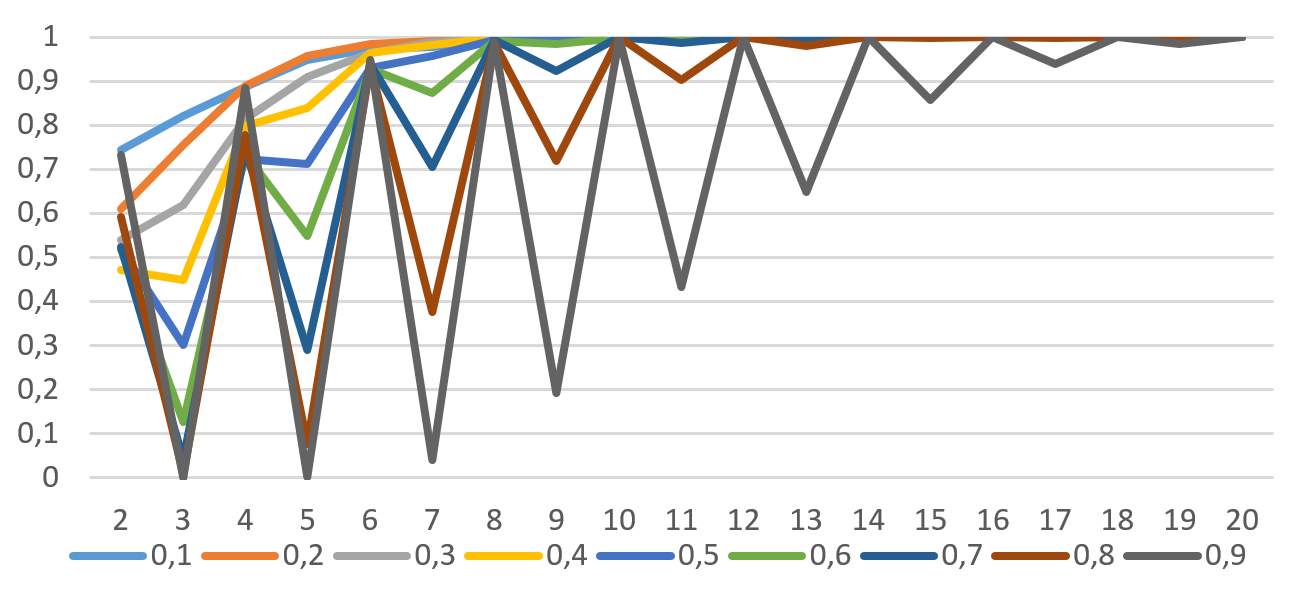
\includegraphics[width=\textwidth]{figures/images/solvabilityOfInputs/binomial_Input_Solvable_m10.png}\label{fig:firstBinPercentage}
      \end{minipage}
      \hspace{0.75cm}
      \begin{minipage}[b]{0.45\textwidth}
            \caption{Percentage of Binomial inputs with perfect partitions for m = 100}
            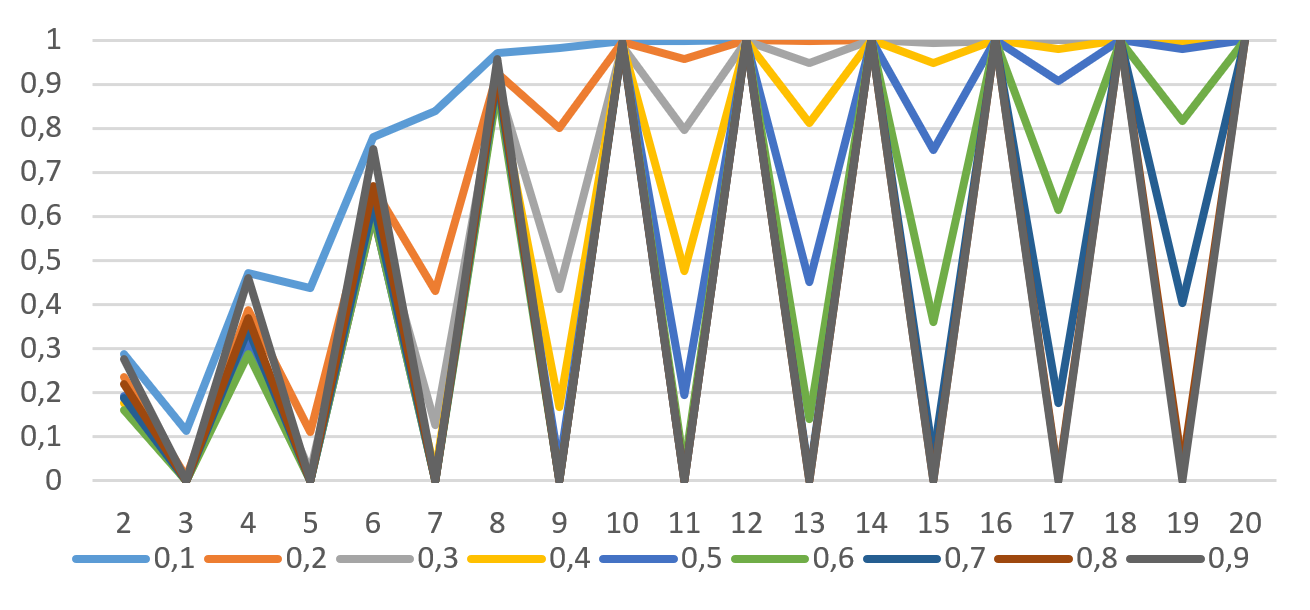
\includegraphics[width=\textwidth]{figures/images/solvabilityOfInputs/binomial_Input_Solvable_m100.png}
      \end{minipage}
\end{figure}

\begin{figure}[h]
      \centering
      \begin{minipage}[b]{0.45\textwidth}
            \caption{Percentage of Binomial inputs with perfect partitions for m = 1000}
            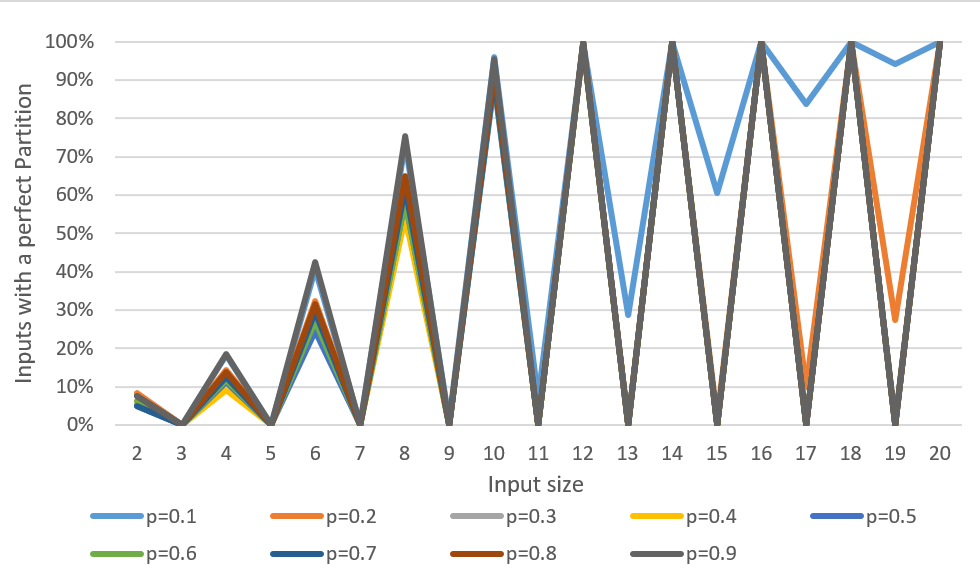
\includegraphics[width=\textwidth]{figures/images/solvabilityOfInputs/binomial_Input_Solvable_m1000.png}
      \end{minipage}
      \hspace{0.75cm}
      \begin{minipage}[b]{0.45\textwidth}
            \caption{Percentage of Binomial inputs with perfect partitions for m = 10000}
            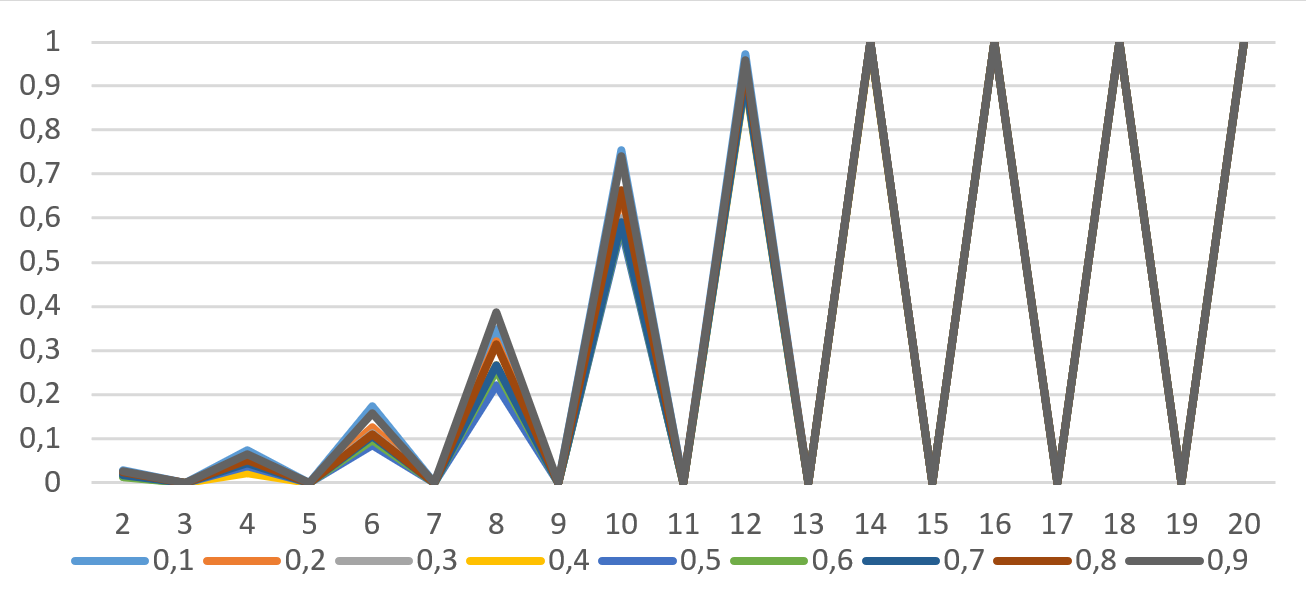
\includegraphics[width=\textwidth]{figures/images/solvabilityOfInputs/binomial_Input_Solvable_m10000.png}
      \end{minipage}
\end{figure}

\begin{figure}[h]
      \caption{Percentage of Binomial inputs with perfect partitions for m = 100000}
      \centering
      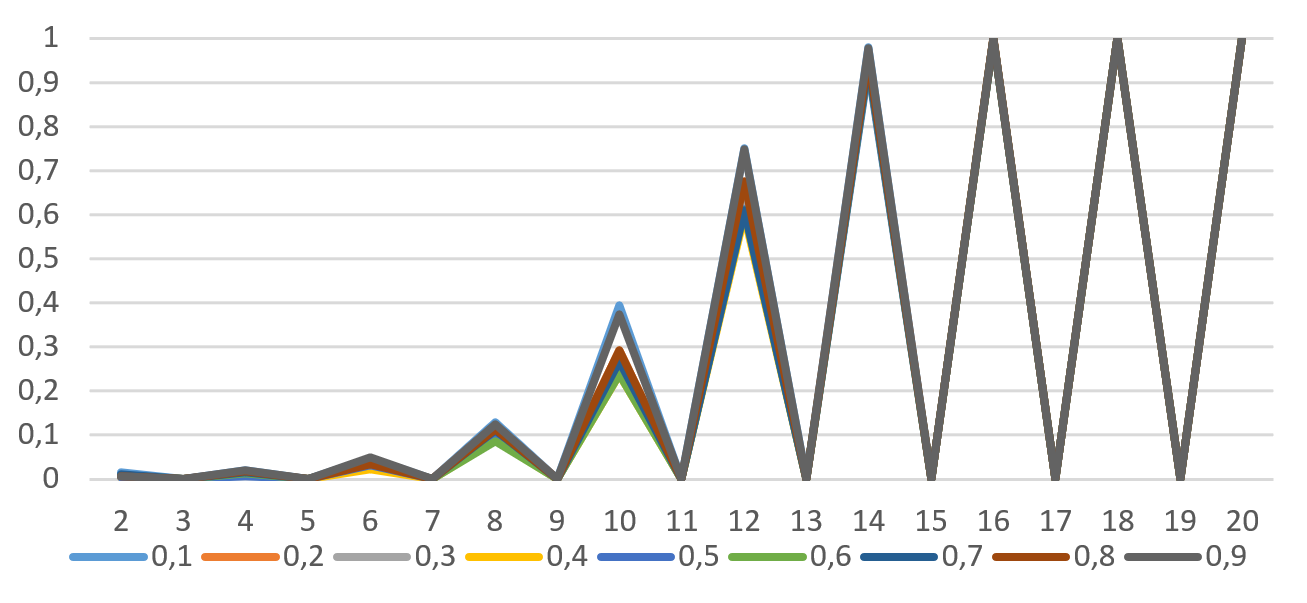
\includegraphics[width=0.45\textwidth]{figures/images/solvabilityOfInputs/binomial_Input_Solvable_m100000.png}\label{fig:lastBinPercentage}
\end{figure}


In the second experiment the inputs were generated a bit differently. Here the goal was to keep the expected value fixed for any combination of $p$ and $n$ and set the value of $m$ to $e/p$ for all $e \in \{10, 20, 30, 40, 50, 100, 200, 500, 1000, 2000, 5000, 10000, 50000\}$. With this setup the influence of the expected value is almost isolated from the other parameters. The probability is still linked $p$ as p also influences the variance $mp(1-p)$. By looking at figure~\ref{fig:firstBinPercentage2} to figure~\ref{fig:lastBinPercentage2} it seems as if the value of $p$ has a much smaller influence than the expected value. For a fixed expected value and a fixed input size a higher value for $p$ seems to increase the percentage of inputs with a perfect partition. 

\begin{figure}[h]
      \centering
      \begin{minipage}[b]{0.45\textwidth}
            \caption{Percentage of Binomial inputs with perfect partitions for p = 0.1}
            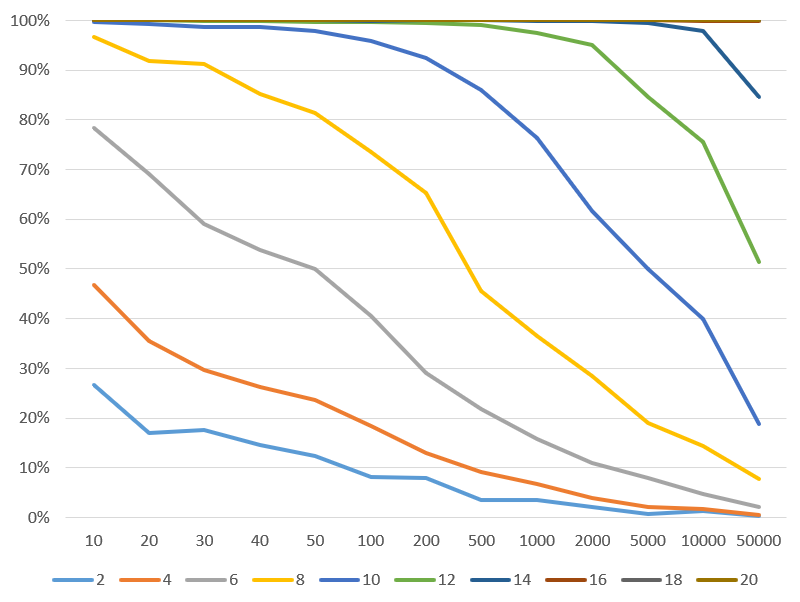
\includegraphics[width=\textwidth]{figures/images/solvabilityOfInputs/solvability0_1.png}\label{fig:firstBinPercentage2}
      \end{minipage}
      \hspace{0.75cm}
      \begin{minipage}[b]{0.45\textwidth}
            \caption{Percentage of Binomial inputs with perfect partitions for p = 0.2}
            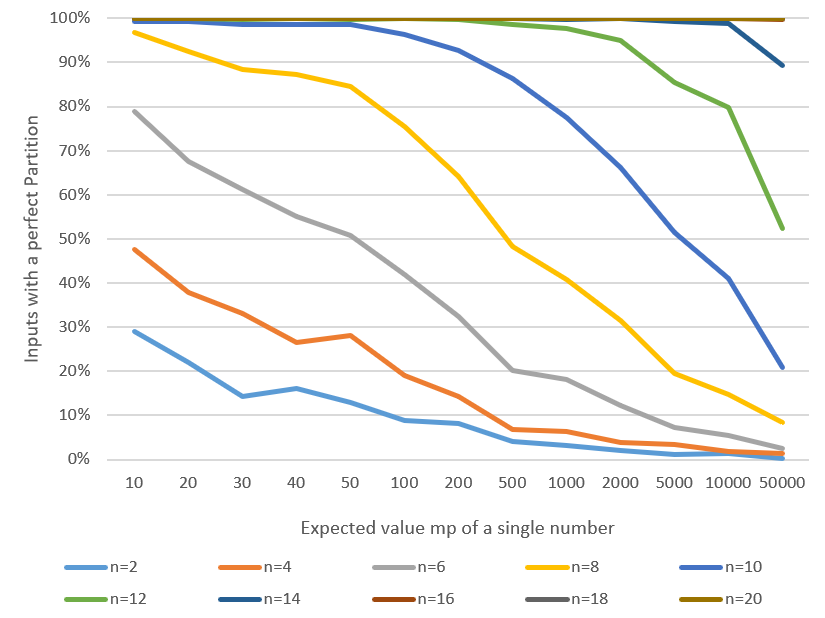
\includegraphics[width=\textwidth]{figures/images/solvabilityOfInputs/solvability0_2.png}
      \end{minipage}
\end{figure}


\begin{figure}[h]
      \centering
      \begin{minipage}[b]{0.45\textwidth}
            \caption{Percentage of Binomial inputs with perfect partitions for p = 0.3}
            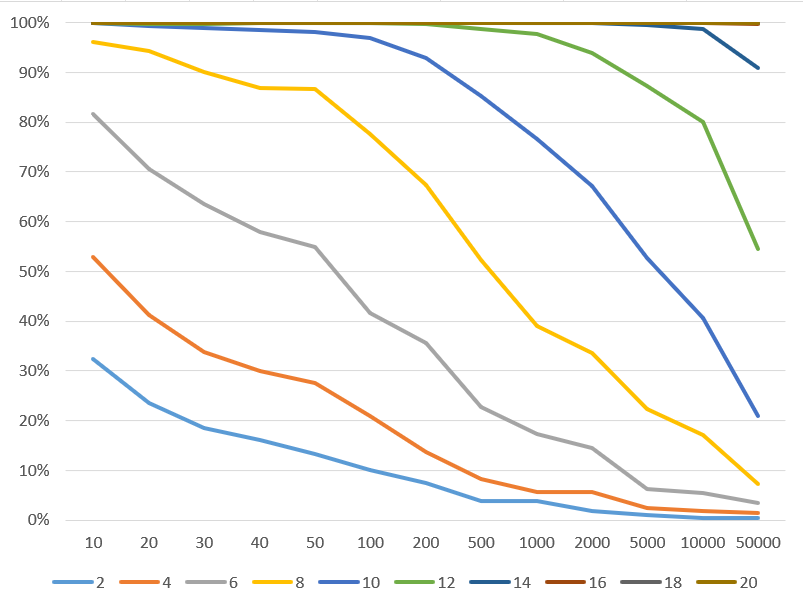
\includegraphics[width=\textwidth]{figures/images/solvabilityOfInputs/solvability0_3.png}
      \end{minipage}
      \hspace{0.75cm}
      \begin{minipage}[b]{0.45\textwidth}
            \caption{Percentage of Binomial inputs with perfect partitions for p = 0.4}
            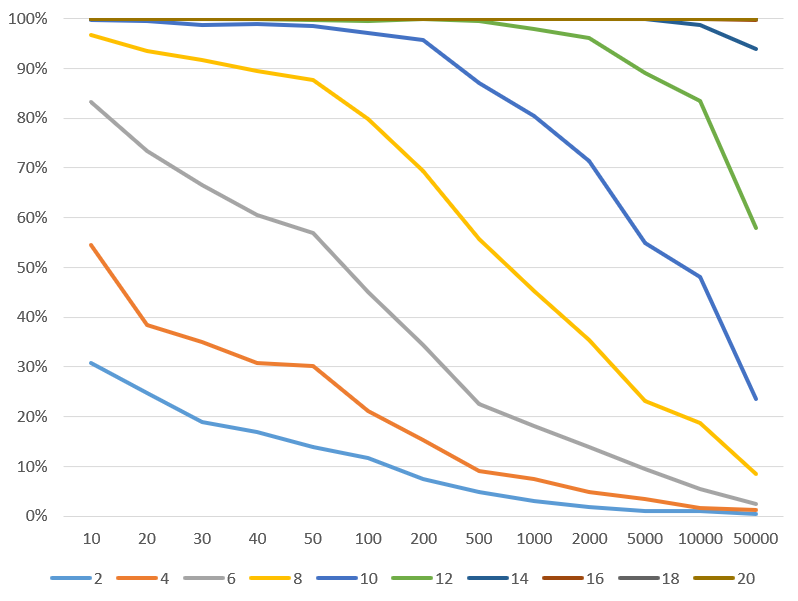
\includegraphics[width=\textwidth]{figures/images/solvabilityOfInputs/solvability0_4.png}
      \end{minipage}
\end{figure}


\begin{figure}[h]
      \centering
      \begin{minipage}[b]{0.45\textwidth}
            \caption{Percentage of Binomial inputs with perfect partitions for p = 0.5}
            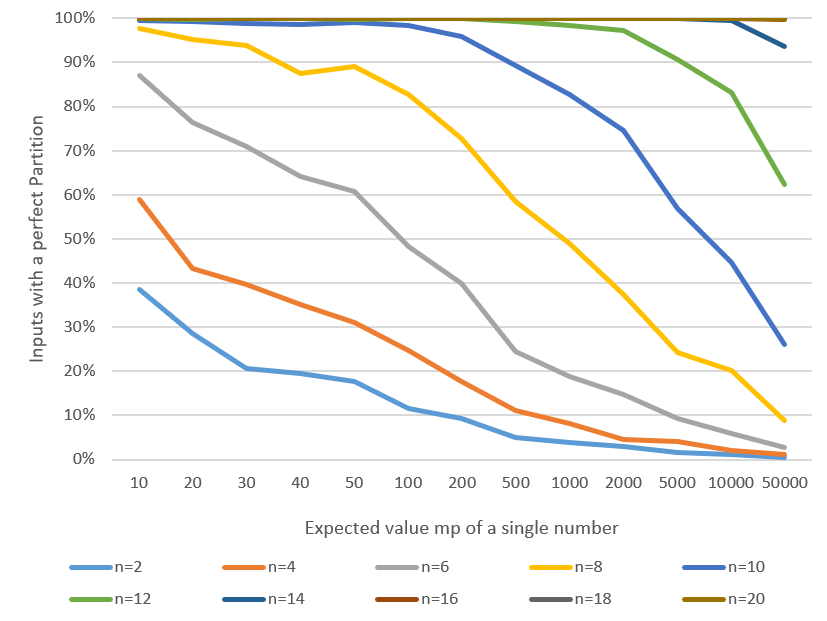
\includegraphics[width=\textwidth]{figures/images/solvabilityOfInputs/solvability0_5.png}
      \end{minipage}
      \hspace{0.75cm}
      \begin{minipage}[b]{0.45\textwidth}
            \caption{Percentage of Binomial inputs with perfect partitions for p = 0.9}
            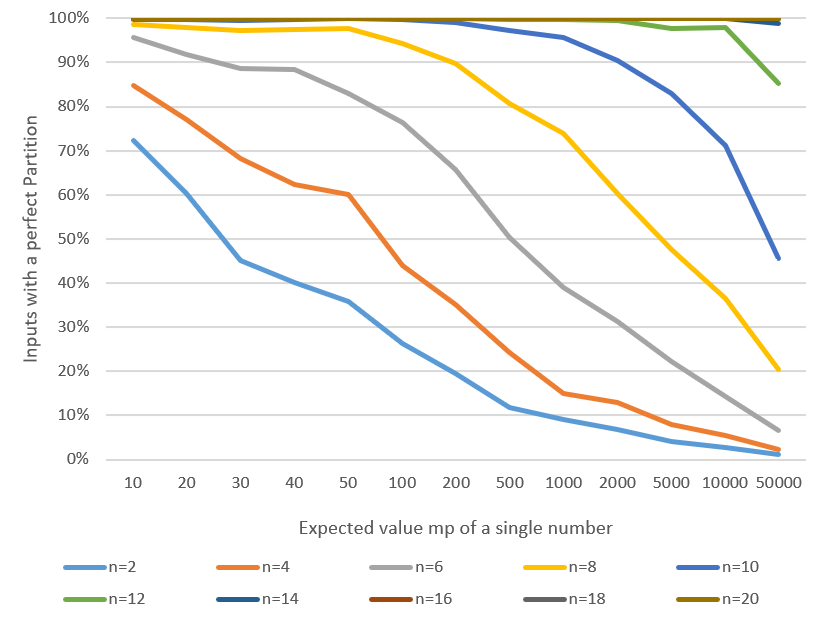
\includegraphics[width=\textwidth]{figures/images/solvabilityOfInputs/solvability0_9.png}\label{fig:lastBinPercentage2}
      \end{minipage}
\end{figure}

\section{Binomial distributed inputs}
\subsection{RLS Comparison}
\subsection{(1+1) EA Comparison}
\subsection{pmut Comparison}
\subsection{Comparison of the best variants}

\section{Uniform distributed inputs}
\subsection{RLS Comparison}
\subsection{(1+1) EA Comparison}
\subsection{pmut Comparison}
\subsection{Comparison of the best variants}

\section{Exponential distributed inputs}
\subsection{RLS Comparison}
\subsection{(1+1) EA Comparison}
\subsection{pmut Comparison}
\subsection{Comparison of the best variants}

\section{OneMax Equivalent for PARTITION}
This kind of input is more or less equivalent to the OneMax problem. All values except the last are either 1 or uniform
random in any intervall. The last value is the sum of all other values. The optimal solution is therefore the 000...01 or
the 111...01 string. So the best solution is almost identical to OneMax. In the previous chapter the O(nlogn) bound was
proven for the (1+1) EA and the RLS. This seems to hold in practice:
TODO: insert Graph showing RLS and (1+1) EA need time O(nlogn)

For OneMax the mutation rate of 1/n is proven to be optimal for the (1+1) EA (TODO insert cite). This seems to be also
true for the equivalent for PARTITION. For Both the (1+1) EA and both new Variants of the RLS
\subsection{RLS Comparison}
The
\subsection{(1+1) EA Comparison}
\subsection{pmut Comparison}
\subsection{Comparison of the best variants}

\section{Carsten Witts worst case input}
\subsection{RLS Comparison}
\subsection{(1+1) EA Comparison}
\subsection{pmut Comparison}
\subsection{Comparison of the best variants}

\section{PowerLawDistributed}
\subsection{RLS Comparison}
\subsection{(1+1) EA Comparison}
\subsection{pmut Comparison}
\subsection{Comparison of the best variants}

\section{Multiple distributions overlapped}
\subsection{RLS Comparison}
\subsection{(1+1) EA Comparison}
\subsection{pmut Comparison}
\subsection{Comparison of the best variants}

\section{Multiple distributions mixed}
\subsection{RLS Comparison}
\subsection{(1+1) EA Comparison}
\subsection{pmut Comparison}
\subsection{Comparison of the best variants}

\section{Multiple distributions mixed \& overlapped}
\subsection{RLS Comparison}
\subsection{(1+1) EA Comparison}
\subsection{pmut Comparison}
\subsection{Comparison of the best variants}
%% conclusion.tex
%%

%% ==================
\chapter{Conclusion}
\label{ch:conclusion}
%% ==================

There is no clear best algorithm for every input for PARTITION and not even a best parameter for every algorithm.
For inputs that are comparable to a linear function/OneMax for all base algorithms the parameter with the lowest mutation rate has the best runtime.
Other instances like the worst case input of C. Witt on the other hand require much higher mutation rates for the optimal performance.
Inputs generated from a powerlaw distribution showed that the optimal parameter for every algorithm is not even fixed within a specific distribution.
For inputs drawn from \textasciitilde$D^{2.75}_{50000}$ the higher mutation rates reached an optimum faster than the lower mutation rate for every algorithm variant.
If the input was drawn from \textasciitilde$D^{1.25}_{50000}$ then the fastest mutation rates for the (1+1) EA on \textasciitilde$D^{2.75}_{50000}$ distributed inputs then instead became the slowest.\newline
So almost no general advice is possible, but a few points still hold for every input type.
The first one is the RLS being most likely to be stuck in a local optimum especially for the smaller input size.
Even if a variant of the RLS is the fastet for the bigger input sizes it is most likely to be stuck in a local optimum for $n\le100$ for most input types.
So if the input size $n\le100$ choosing the (1+1) EA or $pmut$ mutation operator is a better choice.
Another noticeable relation is that inputs that require higher mutation rates are generally easy to solve and are also solved very fast by the lower mutation rates.
A lower number of iterations also does not imply a shorter runtime in every case.
If the mutation rate $1/n$ needs only a few iterations more than $100/n$ it will still be much faster since one iteration is much shorter.
The lower mutation rates are therefore generally a better choice as they will need less time in most cases and are still rather fast if they are not the fastest.
Only if the algorithm is trapped due to its low mutation rate a higher mutation rate makes a huge difference.\newline
Another point is that the Evolutionary Algorithms perform better for larger input sizes as there are more perfect partitions.
The more perfect partition an input has, the easier it is to find one.
For the lower values of $n$ the algorithm sometimes needed 20,000 iterations on average if they managed to find a perfect partition and even longer otherwise.
A runtime of \(100,000\approx2^{14,29}\ge 2^{n-6}\ge2^{n/2}\) is exponential in the size of the input.
So for smaller values choosing other approximation algorithms or even exact algorithms will probably lead to better a better runtime.
For higher values of $n$ on easier inputs they might be efficient as well or in some cases even better.\newline
The last common relation is the less small values especially close to 1 an input has the better flipping 2 or 4 bits in a step becomes.
This was only shown for the binomial distributed inputs but on inputs from \textasciitilde$U(10^4,5\cdot 10^5)$ the results were mostly the same.
To make the thesis shorter this was not listed in the corresponding section.

\begin{table}[t]
      \caption{Best algorithms variants for all evaluated input types}
      \begin{tabular}{c|ccc|ccc|ccc}\label{table:BestAlgoVariantsTable}
                                                   &
            \multicolumn{3}{c|}{RLS variants}      &
            \multicolumn{3}{c|}{(1+1) EA variants} &
            \multicolumn{3}{c}{$pmut$ variants}                                                                                      \\
                                                   & 1st      & 2nd      & 3rd      & 1st     & 2nd    & 3rd    & 1st  & 2nd  & 3rd  \\\hline
            binomial                               & \RLSN[2] & \RLSN[4] & \RLSR[2] & 3$/n$   & 4$/n$  & 2$/n$  & 2.0  & 2.25 & 2.5  \\
            geometric                              & \RLSR[2] & \RLSR[3] & \RLSR[4] & 2$/n$   & 1$/n$  & 3$/n$  & 3.25 & 3.0  & 2.75 \\
            uniform                                & \RLSN[2] & \RLSR[3] & \RLSR[4] & 4$/n$   & 3$/n$  & 2$/n$  & 2.0  & 2.25 & 2.75 \\
            polwerlaw                              & \RLSR[4] & \RLSN[3] & \RLSR[3] & 4$/n$   & 3$/n$  & 5$/n$  & 1.5  & 1.75 & 1.25 \\
            linear function                        & RLS      & \RLSR[2] & \RLSR[3] & 1$/n$   & 2$/n$  & 3$/n$  & 3.5  & 3.25 & 3.0  \\
            worst case                             & \RLSN[4] & \RLSR[4] & \RLSN[3] & 100$/n$ & 50$/n$ & 10$/n$ & 1.25 & 1.5  & 1.75 \\
            combined                               & RLS      & \RLSR[2] & \RLSR[3] & 1$/n$   & 2$/n$  & 3$/n$  & 3.25 & 3.0  & 2.75 \\
      \end{tabular}
\end{table}

Now to round this paper up there are two tables that summarise the previous results.
For each input type and each algorithm the best three variants are listed in Table~\ref{table:BestAlgoVariantsTable} ordered by their average runtime.
This implies a general tendency of better algorithms but is not necessarily a complete insight as the best parameter and algorithm changes depending on $n$.
Table~\ref{table:BestAlgoVariantTable} list my personal preference based on the previous results depending on the distribution and size of the input.
There is no clear overall winner but if one algorithm must be chosen for any input then choosing $pmut_{2.25}$ should be a good option.
For binomial distributed inputs the \RLSN[2] and the \RLSN[4] are the fastest RLS variants but for the OneMax equivalent they need about \(\Theta(\frac{n^k}{k!})\) iterations on average and expectation.
The runtime of the other RLS variants is also too unstable.
So the RLS versions are too much dependent on the input and should not be chosen in every case, especially if the input size is small.
For the best (1+1) EA variants this does not to that extend as the mutation rate $3/n$ is under the top 3 for every input type except the worst case input.
Yet on the OneMax input and the worst case input the (1+1) EA with mutation rate $3/n$ does not reach the optimal solution in all runs in at most $10n\ln{n}$ steps.
$pmut_{2.25}$ is not always one of the best three $pmut$ variants but is also never one of the worst and for the bigger input sizes it also reaches the optimal solution for almost any input in $10n\ln{n}$ steps except for 2/10,000 runs for the Worst Case input of C. Witt.
So if only one algorithm for every input must be chosen, then $pmut_{2.25}$ should be one of the best options.

\begin{table}[h]
      \caption{Suggestions for the fastest algorithm on each input depending on the input size (the (1+1) EA is listed as EA to make the table shorter)}
      % \begin{tabular}{cccccccccc}\label{table:BestAlgoVariantTable}
      \begin{tabular}{m{2.5cm}m{1cm}m{1cm}m{0.5cm}m{0.5cm}m{0.5cm}m{0.5cm}m{0.5cm}m{0.5cm}m{1cm}m{1cm}}\label{table:BestAlgoVariantTable}
            input size $n$  & \multicolumn{2}{|c}{$100$}                          & \multicolumn{2}{c}{$500$}
                            & \multicolumn{2}{c}{$1000$}                          & \multicolumn{2}{c}{$5000$}
                            & \multicolumn{2}{c}{$50,000$}                                                                                         \\
            \hline
            geometric       & \multicolumn{5}{|c|}{EA $_{2/n}$}                   & \multicolumn{4}{c|}{$pmut_{3.25}$} & RLS                       \\
            \hline
            binomial        & \multicolumn{3}{|c|}{EA $_{3/n}$}                   &
            \multicolumn{7}{c}{\multirow{2}{*}{\RLSN[2]}}                                                                                          \\
            uniform         & \multicolumn{3}{|c|}{EA $_{4/n}$}                   & \multicolumn{7}{c}{}                                           \\
            \hline
            powerlaw        & \multicolumn{10}{|c}{$pmut_{1.5}$ or $pmut_{1.75}$}                                                                  \\
            \hline
            linear function & \multicolumn{10}{|c}{RLS}                                                                                            \\
            \hline
            worst case      & \multicolumn{10}{|c}{$pmut_{1.25}$}                                                                                  \\
            \hline
            combined        & \multicolumn{1}{|c|}{EA $_{2/n}$}                   & \multicolumn{6}{c|}{$pmut_{3.25}$} & \multicolumn{3}{c}{RLS}   \\
                            &                                                     &                                    &
                            &                                                     &                                    &
                            &                                                     &                                    &                         & \\
      \end{tabular}
\end{table}



%% --------------------
%% |   Bibliography   |
%% --------------------

\cleardoublepage
\phantomsection
\addcontentsline{toc}{chapter}{\bibname}

\iflanguage{english}
{\bibliographystyle{alpha}}
{\bibliographystyle{babalpha-fl}} % german style

\bibliography{references}


%% ----------------
%% |   Appendix   |
%% ----------------

\cleardoublepage
%% appendix.tex
%%

%% ==============================
%\chapter{Appendix}
%\label{ch:Appendix}
%% ==============================

\appendix

\iflanguage{english}
{\addchap{Appendix}}	% english style
{\addchap{Anhang}}	% german style


\section{Appendix Section 1}
\label{appendix1}

\begin{figure} [ht]
  \centering
   ein Bild
  \caption{A figure}
  \label{fig:BPMNBeispiela}
\end{figure}




\end{document}
